\documentclass[twocolumn]{article}
\usepackage{color}
\usepackage{multirow}  
\usepackage{listings}
\usepackage{float}
\usepackage{amsfonts}
\usepackage{amssymb}
\usepackage{amsmath}
\usepackage{cite}
\usepackage{listings}
\usepackage{xcolor}
\usepackage{graphicx}
\usepackage{draftwatermark}
\SetWatermarkText{DRAFT YELLOW PAPER}
\SetWatermarkScale{1}
\definecolor{pagecolor}{rgb}{1,0.98,0.9}
\pagecolor{pagecolor}
\setlength\parskip{.5\baselineskip}
\author{Ryan J. Kung \\ryankung@ieee.org\\Member, IEEE Blockchain Community }
\title{Inferred based Distributed Gaming and Nash Equilibrium}
\begin{document}
\maketitle
% \tableofcontents
\section{Abstract}
Since the introduction of Ethereum on 2014\cite{ethereum}, It brought many DApps and DGames, such as CryptoKitty, Etheremon and Decentraland. Most of them were running into issues addressed to the congestion of transaction which is limitation of how Ethereum implemented. Storing on-chain data is too expensive for games needs high interaction, and may cause may problem, one of them is that gaming on distributed system may cause harder to find out a fear nash equilibrium point for numerical designing, and the nonnegligible delay of tranasction caused may limited the interactive rate of game processing.

In this paper, we studied and discussed how should a distributed game works on blockchain based distributed system. First, we discussed distributed nash equilibrium problem on certain condition, then we introduced an infered based system based on an abstraction which formalize blockchain with STMonad and Lens application, further, we discussed how to composed infered system with zero-knowledge proof for game refining.

\section{Distributed Gaming}


Like traditional Gaming on game theory, we defined DGaming as a series of Gaming Behaviors and Strategis which is Distributed. With Lamport's defination on 1978\cite{time-clocks-ordering-events-distributed-system}, A Gaming is Distributed if the message transaction delay is not negligible compared to the time between event in classic gaming behavior.
\subsection{Nash Equilibrium Seeking}
Traditional gaming theory may easily lead us run into issues if it's distributed, such as nash equilibrium simulation or prisoner's dilemma problem.

On classic Nash Equilibrium, we seek out the nash-eq point by analyze it with action matrix, and proof that for each strategy on game $(S, f)$, and got A strategy profile which is Nash Equilibrium. But on distributed case, the issue is that the event of strategy is not effect immediately, nonnegligible delay of transaction on system may cause N-Eq point out of expectation.

For example, we discuss a classic game as:
\begin{center}
\begin{tabular}{c|c|c|}
  & L & R \\
  \hline
  U & (1,3)&(-3,0)\\
  \hline
  M & (-2,0)&(1,3)\\
  \hline
  D & (0,1)&(0,1)\\
\end{tabular}
\end{center}

With Repeated advantage solution, we can simply figure out that the nash-eq strategy is $(U, L)$, but this game is based on a hypothesis that player $i$ shares same knowledge about payoff and strategy space. If players are sensitive on the uncertainty of $s_{-1}$, they may not choose the rational strategy, like if about \%1 players choose $R$, then $D$ is better than $U$.


\begin{figure}[H]
  \centering
  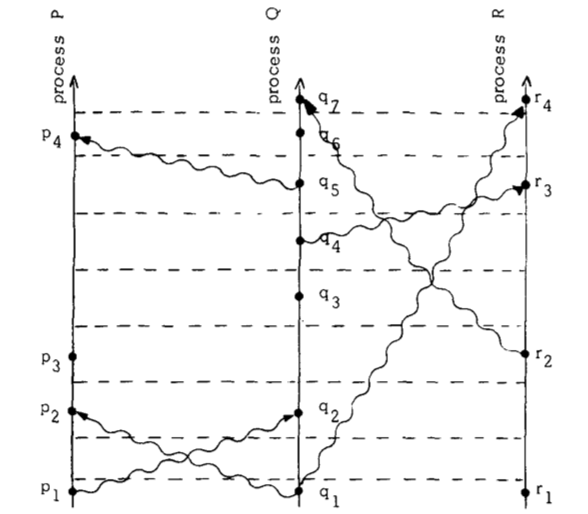
\includegraphics[width=0.5\linewidth]{img/lamportts.png}
  \caption{Lamport Timestamp}
\end{figure}


In distributed game, for example an distributed game based on a paxos based system. Addressed to the nonnegligible delay, player $i$ may upfront know $i'$ and action hysteretic, which may cause the nash-equilibrium become highly dependents on the distributed network. Figure 1 is showing that how events can be trigger and measured on a distributed system. Actually, on a Dgame all players may tried to mining more informations and action as later as they can, the situation may looks like Prisoners’ Dilemma:

\begin{center}
\begin{tabular}{c|c|c|}
  & W & A \\
  \hline
  W & (1,1)&(-1, 2)\\
  \hline
  A & (2,-1)&(0,0)\\
\end{tabular}
\end{center}

On this game, players can choose from strategy space ${Wait, Action}$, and as what prisoner's dilemma presented to us, all players may choose $W$. Which entangled the gaming into a series complicated case, and break perfect information gaming in to imperfect.


 Nash equilibrium seeking under communication networks is as tracing increasing attension resently, The distributed equilibrium seeking strategy(DESS) was given by \cite{7888532}:
\begin{gather}
  \dot{x} = k_i \frac {\partial f_i}{\partial x_i}(y_i), i \in \mathbb{N}
\end{gather}

T$(\dot{x}^*, 1_N\oplus x^*)$, where $x^*$ presents nash equilibrium. There exist Some seeking work on it with paritially coupled payoff method\cite{8029164}, or Communication Topologies\cite{8093754} building on certain conditions and developed on the discrete-time stochastic algorithm\cite{928588} which the players are supposed to be capable of communicating with each other via an undirected and connected communication graph\cite{7888532}. 

\subsection{Formulation}
In the game we designed, there are two tokens:

1. {\bfseries Premier}: An Exchangeable ERC20 token, which can exchange with Ether and have a dynamic inflation rate $\Delta \mathbb{S}$, based on total number of player $I$ on lamport timestamp $t$:

\begin{gather}
  \Delta \mathbb{S}(t) = f \circ I (t) \\
  \Delta \mathbb{S}(t) > \Delta \mathbb{S}(t') \iff I(t) < I(t')\\
  \Delta \mathbb{S}(t) = \Delta \mathbb{S}(t') \iff I(t) = I(t')\\
  \Delta \mathbb{S}(t) < \Delta \mathbb{S}(t') \iff I(t) > I(t')
\end{gather}

And the total supply $\mathbb{S}$ on lamport timestamp $t$ is:

\begin{gather}
  \mathbb{S}(t) = \sum_{i=0}^t f \circ I(t)
\end{gather}

For Premier Token, the strategy space is:

\begin{gather}
  S_{premier} = \{B, S, H, G\}
  \intertext{Where:}
  \begin{tabular}{c    l}
    B:= & \text{Buy Premier from Exchange}\\
    S:= & \text{Sell Premier to Exchange}\\
    H:= & \text{Hold Premier and do noting}\\
    G:= & \text{Gaming for Reward Token}
\end{tabular}\nonumber
\end{gather}

2. {\bfseries Reward}: An Exchangeable ERC721 token which is delegated with premier by strategy $G$. When players do Gaming, there is a probability $P$ for reward getting, based on total number of player $I$ who do game. The expected value of Reward inflation rate is:

\begin{gather}
  E(t) = I(t) \cdot P \circ I (t) \\
  P(t) > P(t') \iff I(t) < I(t')\\
  P(t) = P(t') \iff I(t) = I(t')\\
  P(t) < P(t') \iff I(t) > I(t')
\end{gather}

For Premier Token, the strategy space is:

\begin{gather}
  S_{reward} = \{B, S, H\}
  \intertext{Where:}
  \begin{tabular}{c    l}
    B:= & \text{Buy Reward from Exchange with Premier}\\
    S:= & \text{Sell Reward to Exchange for Premier}\\
    H:= & \text{Hold Reward and do noting}\\
\end{tabular}\nonumber
\end{gather}

And the total supply $\mathbb{S}$ on lamport timestamp $t$ is:

\begin{gather}
  \mathbb{S}(t) \approx \sum_{i=0}^t E(t)
\end{gather}


\section{Infered Game}


On case on time $t$, we have a active matrix, player 1, 2 can Gaming, Holding or Selling. Addressed to formular $(2), (3), (4)$, if 1, 2 all do gaming, they will get less payoff, and due to the inflation rate, if 1, 2 just holding, they will lose money which relative to. And if 1 is gaming, and 2 is Selling, because of the decreasing of total supply, seller will get more profit:

\begin{gather}
\begin{tabular}{c|c|c|c|}
  & G & H &S\\
  \hline
  G & (1, 1)&(2, -1)&(2,2)\\
  \hline
  H & (1, 2)&(-1, -1)&(-2, 1)\\
  \hline
  S & (2,2)&(1,0)&(0, 0)\\
\end{tabular}
\end{gather}

With PAS:

\begin{gather}
\begin{tabular}{c|c|c|}
  & G &S\\
  \hline
  G & (1, 1)&(2,2)\\
  \hline
  S & (2,2)&(0, 0)\\
\end{tabular}
\end{gather}

In this paper, we considered a game $(S, f)$ with a set of player $\mathbb{N} = {1, 2, ..., N}$, under a distributed network which has nonnegligible delay $\mathbb{\delta}$, all player $i$ can well access actions of $-i$. We define a mix strategy function $\sigma = f(\delta, s)$ which is means how the information is prefect for $s_i$. And formulated the mix strategy function based on nonnegligible transaction as $sigma(\delta, \dot{x})$.

If $\delta$ for DGame $(18)$ is negligible, $(\sigma(G), \sigma(S))$ should be $(\frac{1}{2}, \frac{1}{2})$, otherwise player $i$ may known the action $-i$ does early, which may shifts the distribution to $(0, 1)$. And if most of players does same, it will fall into a zero-sum game trap. We introduce infered game for solving this problem.

\subsection {STMonad and Lens}

An infered Game is that for a game (S, f), all players $i$ shares same knowledge space about $S$, $u_{i}(s)$, and $s_{-i}$ on  Lamport Timestamp $\tau$.
Unlike classic distributed system,
Since some formalization of blockchain is based on the separation logic or $\pi calculis$ \cite{linearblockchain}, it can easily be modeled as a time step function, or a FRP issue which can be abstract as\cite{ElliottHudak97:Fran}, where blockchain Status can be also be abstract as $STMonad$ like MAKERDao\cite{dai}'s work:

\begin{gather}
  time: STMonad_{time}\\
  at \mathbb{[} time \mathbb{]}t = t
\end{gather}

In blockchain, there is only one types of monad, the STMonad, $STMonad$ is a Monad type for status, thus except status changes, all other functions should be pure which means no side-effect, which means we can build an infered system or a $LENS$\cite {lens} above it. A Lens should have two property, $over$, and $view$. 

\lstset{language=Haskell}
\begin{lstlisting}
data Lens a b = Lens
    { view :: a -> b
    , over :: (b -> b) -> (a -> a)
  }
\end{lstlisting}

\subsection {Consistency of Blockchain}

In solidity, a pure function which means nor cost gas or cause side-effect on blokchain it can be infered based on ABI is a $Lens.view$, otherwise it's a $Lens.over$ which means you have to send a transaction to modified the status of chain.

Consider the Gaming strategy $G$, on time $t$, all players i should know $I(t)$ as $Lens.view$, and calculate out the utility function of selling or mining with $q$ tokens with cost $c$:

\begin{gather}
  u(q_i) = q_ip(q) - c_i(q_i)\\
  p(q_i) = f(\mathbb{S}(t))
\end{gather}

Like cournot duopoly model, with a two player $\{1, 2\}$ gaming, we can directly give the nash equilibrim of $S$ is:

\begin{gather}
  \dot{q}_1 = \dot{q}_2 = \frac{1-c}{3}
\end{gather}

And when $i$ trying do action, it's a $Lens.over$ which overwrite the status of contract storage. Based on the Infered system, $-i$ can access $S_i$, so as matrix presented in $18$, $-1$ will prefer to select $S$ which means higher payoff. Actually according to symmetry, when $i$ choose $S$, $-i$ will always choose $G$, so that $\sigma$ should be $(\frac{1}{2}, \frac{1}{2})$ which is as same as single-process gaming.

So since classic distributed gaming may transfer the gaming from perfect information to imperfect. But if it's blockchain based, since $over$ is working as eventual consistency\cite{consis} but the status of blockchain can be seems as strong consistency\cite {Consistent}. On $view$ phase of gaming, when player $i$ make decision on $STMonad \  time_0$, the information of $Monat$ is perfect. For phase $over$, players may choose to pay high price as strategy to get more payoff, since it's based on consistency information of blockchain, we can also say that the $over$ phase is also perfect information gaming. So for a gaming we wished to have a fixed nash equilibrium point, it should be designed as all data in public and no private status.

\subsection {Zero Knowledge Game}

Such as we can formalize blockchain as a Monad (A monoid in the category of endofunctors), We can also describe abstractly the cryptology part of bitcoin as a cyclic subgroup of elliptic curve group over a primer finite field, which is also the principle of zk-SNARKs. There is an concrete implementation in our game for providing zero-knowledge proofing based on the infered system and hash algorithms, It's works like other blockchain implementation does \cite{zcash}. But what further more is, we tried developed algorithms based on Abstract Algebra Type and Isomorphism or Bijection mapping.

The Abstract Algebra Type made an allowance for playing high abstract part of calculators in a more intuitionistic way. Such as when we try to implement ethereum's pubkey/privatekey algorithm, we can just simply write as\cite{klefki}:

\lstset{language=Python}
\begin{lstlisting}
  def pubkey(priv: CF) -> ECG:
      return ECG(G @ priv)
\end{lstlisting}

Where CF and ECG is Finite Field Cyclic Group and Elliptic Curve Group of Secp256k1. By the property of cyclic subgroup, we can easily improve the zero knowledge gaming as some endomorphism feature.

\begin{gather}
  A + B = X \\
  A + C = X \\
  C \neq X
\end{gather}

\section {Concrete}

We abstract the gaming activity as mining, and designed a series of numerical system, which can maintain the value of user actor by a fixed and well-designed nash equilibrium pointed.

\subsection {Infered based Token}

The ERC20 standard was extended with a built-in transparen exchange, which makes all gaming actor can be limited inside the blockchain or contract. And based on ERC721, we designed a reward system to keep player can get payoff if they act around the nash-eq point. For Exchangeable ERC20 and so on the Exchangeable ERC721, all matching stuffs is based on infered system, which means players can check the full depth of ticker for determining the best price they should pay for tokens.

Functions of smart contract are separated into Functor and Monad. Functors are working based on pre-infered system, and Monads are based on infered system, which is actually presented a sequence of status.

We support below ABIs:

\begin{gather}
\begin{tabular}{l|l|l}
  function & type & event\\
  \hline
  checkBidTicker & \multirow{4}*{Lens.view} & \multirow{4}*{False} \\
  checkAskTicker& \\
  matchBid & \\
  matchAsk &\\
  \hline
  ask & \multirow{6}*{Lens.over} & \multirow{6}*{True} \\
  bid & \\
  fillBid & \\
  fillAsk &\\
  cancelAsk & \\
  cancelBid & \\
\end{tabular}
\end{gather}

On out implementation of Gaming Token, we designed an infered based auto expended rate. The expand rate is based on $I(t)$ and $time$ of blockchain, which is bounded on the nash equilibrim of what the token price should be during the game processing.

In contract PremierToken.sol, we developed a functional modifier for infered system, which works like a lazy evaluation. Above on ERC20 standard, there is two kind of balance:

1) infered balance

Infered balance is $Lens.view$ which implement a measurement of the real balance should be. If a function is $Lens.view$, it will check infered balance, else it will evaluation the infer modifier and setup infered value to storage of contract.

2) real balance

Real balance is also $Lens.view$ which is just returning real the balance in storage which is excluded infered value.

Standard function transfer, transferfrom and approve are all modified by Infered modifier.

\subsection {Non-fungible Token}

The most obviously case of nash-eq case on blockchain world is bitcoin mining\cite{bitcoin}, we can easily build an game matrix model on bitcoin mining behavior, the relationship is between market force, difficult rate, and hash rate. And in game, players can pay game token for wining reward, more token they paid, higher rewarding rate they got, which is working as a simulation of how bitcoin mining works. The Reward token is a ERC720 token, which is also mapping to IPFS hash address. Like Premier Token, Reward token also has it's expand rate which is based on $I(t)$ and $t$. When gaming, reward token can be immediately infered by the context like tx Hash, sender address or blocktime of blockchain Premier token paid.

For increasing value of NFT Reward Token, we designed several artwork for each logic layer of token which is storing on IPFS, which can be composed in front end of DApps for print and Zero-knowledge Transfer.

A Zero-knowledge Transfer is a transfer with zero context, which is simply developed on freeze and unfreeze strategy. When user transfer Reward Token with Zero-knowledge Transfer, the token id will be freezed on contract for a unique untraceable hashid thus receiver can redeem the hashid that has no idea where the Token is come from.


\section {Conclusion}

Addressed to the strong consistency property of blockchain, A game can have a certain nash equilibrium point, if the side-effects and pure-functions are in separation. 
\bibliographystyle{plain}
\bibliography{dgaming}
\end{document}
